\documentclass{article}  
\usepackage{amsmath}
\usepackage{hyperref}
\usepackage[utf8x]{inputenc}

% Footnote related
\usepackage[bottom]{footmisc} %Footnotes in Tables. Load this before hyperref
\usepackage{graphicx, float, tikz-cd, xcolor, subcaption, chemfig} %Figures and Graphics
\graphicspath{{figures/}}
\usepackage{caption, tabularx, multirow, threeparttable, float} %Tables related
\usepackage{amsmath, amsfonts, amssymb, mathtools, calc} %Maths and Equations
\usepackage{standalone} % load only in the main file
\usepackage{fancyhdr} %For header
\usepackage{emptypage} % Removes header from empty pages
\usepackage{longtable} % Multipage Tables
\usepackage{booktabs} % To use toprule, midrule and bottomrule
\usepackage{makeidx} %To make index page
\usepackage[totoc]{idxlayout} %To get index into TOC
\usepackage[acronym,toc]{glossaries} %Acronyms, TOC option will add it to TOC
\usepackage[titletoc,title]{appendix} %For Appendix
\usepackage{titlesec}
\titleformat{\chapter}[display]
  {\normalfont\sffamily\huge\bfseries\color{black}}
  {\chaptertitlename\ \thechapter}{20pt}{\huge}
\titleformat{\section}
  {\normalfont\sffamily\large\bfseries\color{black}}
  {\thesection}{1em}{}
\usepackage[a4paper,includeheadfoot,margin=2.54cm]{geometry}
\usepackage[version=3]{mhchem} %Chemistry reactions

                            
\title{Spatial models for public health and economic strategies for COVID-19}  
\author{KI, SK, AB, MR}    
\date{\today}     

%% It is just an empty TeX file.
%% Write your code here.

%new definitions
\def\be{\begin{equation}}
\def\ee{\end{equation}}
\def\bea{\begin{eqnarray}}
\def\eea{\end{eqnarray}}
\def\bsplit{\begin{split}}
\def\esplit{\end{split}}

\def\p{\partial} 
\def\nn{\nonumber}
\def\f{\frac}
\def\dbdt{\frac{d}{dt}}

\def\fc{\vartheta} % stress fluctuations
%\def\th{\theta} % stress fluctuations

\def\red{\textcolor{red}}
\def\blue{\textcolor{blue}}

\def\({\left(}
\def\){\right)}
\def\L{\left[}
\def\R{\right]}
\def\la{\langle}
\def\ra{\rangle}
\def\bs{\boldsymbol
}\def\ddx{\partial_x}
\def\ddxx{\partial^2_x}
\def\ddt{\partial_t}
\def\dx{{\dot x}}
\def\dz{{\dot z}}
\def\bx{{\bar x}}
\def\dbx{{\dot \bx}}
\def\dx{{\dot x}}
\def\m{\Delta\mu}
\def\e{\epsilon}
\def\Mbar{\overline{M}}
\def\ldot{\dot{\ell}}
\def\ldotbyl{\frac{\dot{\ell}}{\ell}}

\def\Roo{R_1^{(1)}}
\def\Roz{R_0^{(1)}}

\newcommand{\taumass}{\hat{\tau}_m}
\newcommand{\refn}[1]{Eq. (\ref{#1})}
\newcommand{\pa}{\partial}


\newcommand{\ip}[2]{(#1, #2)}
                             % Defines \ip{arg1}{arg2} to mean
                             % (arg1, arg2).

\begin{document}             

\maketitle                   

%\section{A short excurison into SIR models} 
%
%Richard Neher's model \cite{NeherFeb2020}
%\begin{eqnarray}
%\dbdt S_a &=& -\beta(t) S_{a}(t) \sum_b I_b(t) \\
%\dbdt E_a &=& \beta(t) S_{a}(t) \sum_b I_b(t) - E_a(t)/t_l \\
%\dbdt I_a &=& E_a(t)/t_l - I_a(t)/t_i \\     
%\dbdt R_a &=& m_a I_a(t)/t_i + (1-c_a)H_a(t)/t_h \\
%\dbdt H_a &=& (1-m_a)I_a(t)/t_i + (1-f_a)C_a(t)/t_C \\
%\dbdt C_a &=& c_a H_a(t)/t_h - C_a(t)/t_c \\
%\dbdt D_a &=& f_a C_a(t)/t_c
%\end{eqnarray}
%
%where age index, $a = 1,2,...,9$ standing for age categories: $0-9, 10-19,..., 80+ $.
%
%\[ \beta_a(t) = R_0 \zeta_a M_(t) (1 + \varepsilon\,cos \( \frac{2\pi(t-t_{max})}{t_i} \) \]
%
%\begin{table}[H]
%  \centering
%  \begin{tabular}{l r c l}
%    \toprule
%    \textbf{Parameter} & \textbf{Symbol} & \textbf{Value} & \textbf{Units} \\
%    \midrule
%    avg interactions per day & $R_0$ & 2-3 & per day \\
%    degree of isolation & $\zeta_a$ & 0-1 &  \\
%    mitigation & $M(t)$ & 0-1 &  \\
%    seasonal driving & $\varepsilon$ & 0 & \\
%    peak of seasonal effects & $t_{max}$ & Jan 2020 & time \\ 
%    average latency period & $t_l$ & 5 & days \\
%    average infectious period & $t_i$ & 3 & days \\
%    average hospitalisation time & $t_h$ & 4 & days \\
%    average time in ICU & $t_c$ & 14 & days \\
%    proportion of mild symptoms & $m_a$ & 0-1 & \\
%    proportion requiring critical care & $c_a$ & 0-1 & \\
%    proportion for which the disease is fatal & $f_a$ & 0-1 & \\
%    \bottomrule
%  \end{tabular}
%  \caption{Parameters in the model}
%  \label{table:model_parameters}
%\end{table}
%
%\begin{table}[H]
%  \centering
%  \begin{tabular}{l c c c c c c c c c}
%    \toprule
%    Age groups: & 0-9 & 10-19 & 20-29 & 30 -39 & 40-49 & 50-59 & 60-69 & 70-79 & 80+ \\
%    \midrule
%    $m_a$ & 0.9995 & 0.9985 & 0.997 & 0.9955 & 0.988 & 0.975 & 0.925 & 0.86 & 0.75 \\
%    $c_a$ & 0.05 & 0.1 & 0.1 & 0.15 & 0.2 & 0.25 & 0.35 & 0.45 & 0.55 \\
%    $f_a$ & 0.3 & 0.3 & 0.3 & 0.3 & 0.3 & 0.4 & 0.4 & 0.5 & 0.5 \\
%    \bottomrule
%  \end{tabular}
%  \caption{Age-specific parameters in the model}
%  \label{table:age_specific_parameters}
%\end{table}
%
%\begin{figure}[H]
%    \centering
%    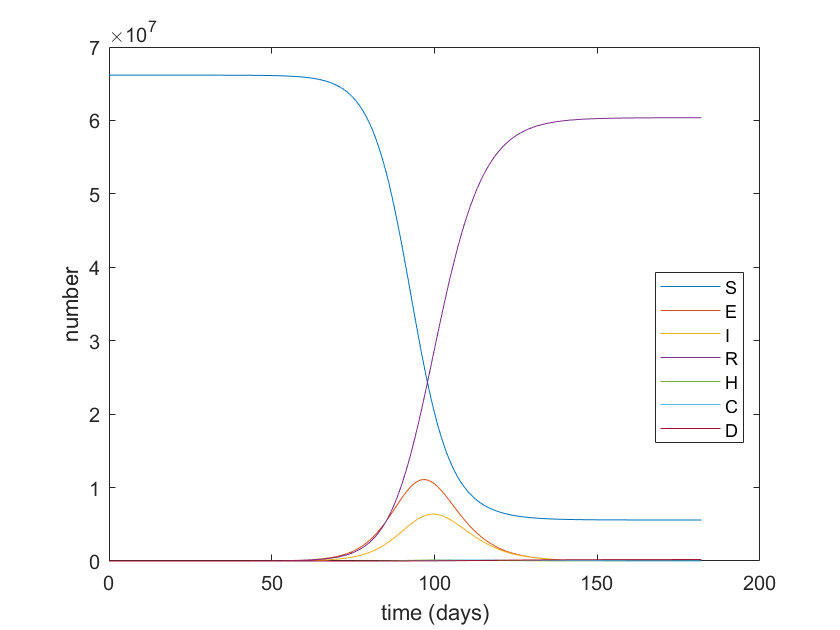
\includegraphics[width=0.45\textwidth]{../../neherlab-comparison/real-time-plot-1}~
%    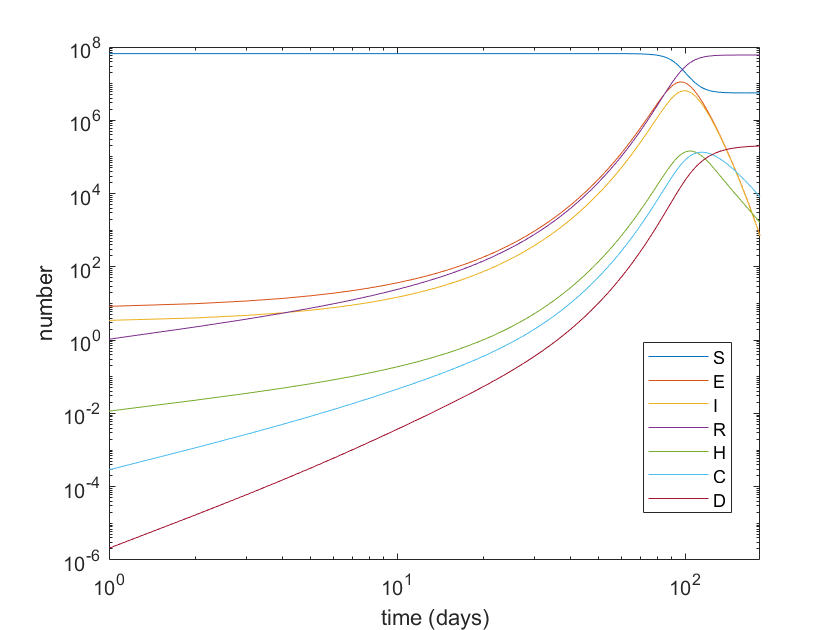
\includegraphics[width=0.45\textwidth]{../../neherlab-comparison/log-log-plot-1}
%    \caption{Test run for Karnataka with a population $N = 66165886$ and initial exposed/infected population of 10, i.e. $E_4 = 7$, $I_4 = 3$ with no mitigation, no imports.}
%    \label{fig:dynamics-no-mitigation}
%\end{figure}
%
%\begin{figure}[H]
%    \centering
%    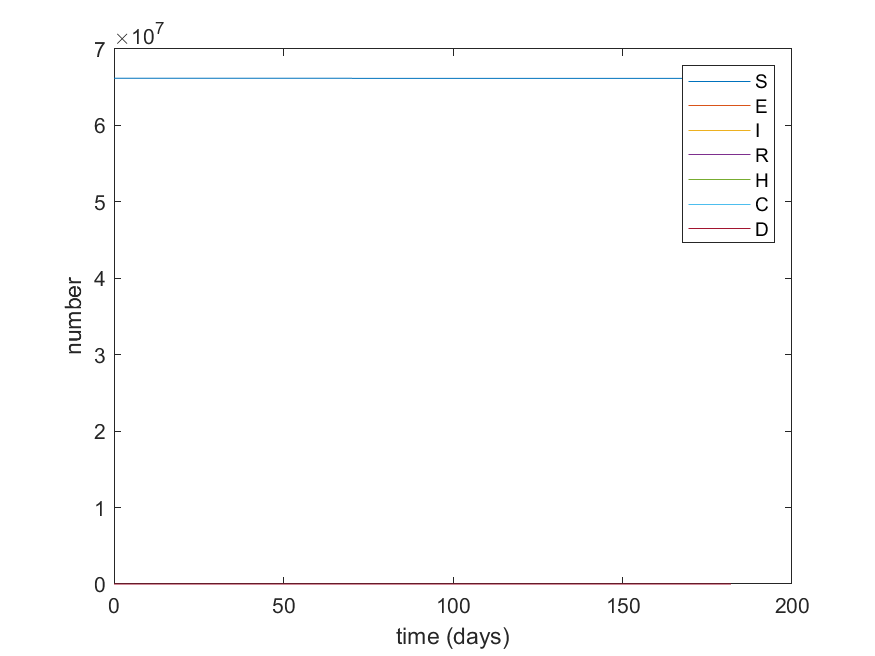
\includegraphics[width=0.45\textwidth]{../../neherlab-comparison/real-time-plot-2}~
%    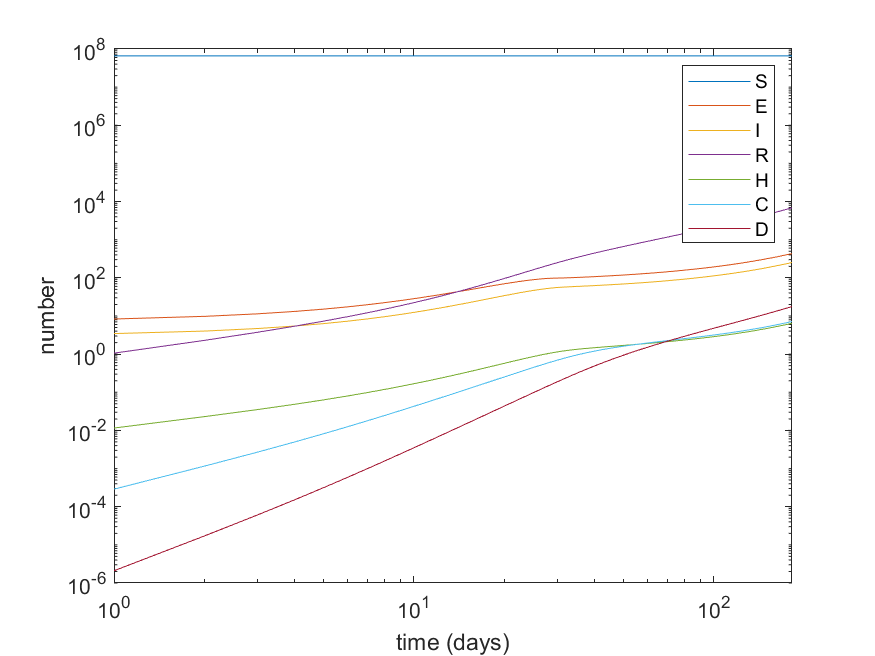
\includegraphics[width=0.45\textwidth]{../../neherlab-comparison/log-log-plot-2}
%    \caption{Test run for Karnataka with a population $N = 66165886$ and initial exposed/infected population of 10, i.e. $E_4 = 7$, $I_4 = 3$ with strong mitigation, no imports}
%    \label{fig:dynamics-strong-mitigation}
%\end{figure}
%
%
%\begin{figure}[H]
%    \centering
%    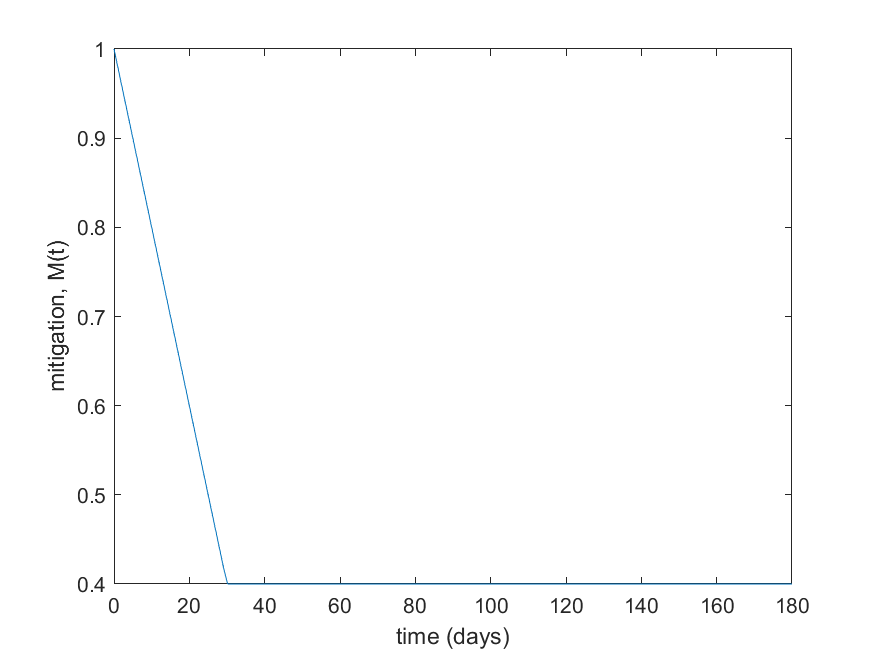
\includegraphics[width=\textwidth]{../neherlab-comparison/strong-mitigation}
%    \caption{Mitigation curve for Fig.\,\ref{fig:dynamics-strong-mitigation}}
%\end{figure}


\section{Our model including economic demographic}

In our model we consider a city and several, $n_v$, villages. 
In each of them the population is divided into:
\begin{enumerate}
	\item 3 economic categories: immobile poor, mobile poor and rich
	\item 3 age categories: children (0-14), young (15-59) and old (60+) 
	\item 5 states:  Susceptible (S), Exposed (E), Infectious (I), Recovered (R), Dead (D)
\end{enumerate}

While we will label the states with a capital letter as indicated next to the states in the list above, we will use a subscript to denote age (a) and economic (e) categories. Therefore, $S_{ae}, I_{ae},...$ such that \[ N(t) = \sum_{a,e} N_{ae}, \qquad N_{ae} = S_{ae}(t) + E_{ae}(t) + I_{ae}(t) + R_{ae}(t) +D_{ae}(t) \] for a city and villages individually. The dynamics is described by the following reaction graph:

\begin{figure}[H]
	\centering
	\includegraphics[width=\textwidth]{scheme2}
\end{figure}

\begin{figure}[H]
	\centering
	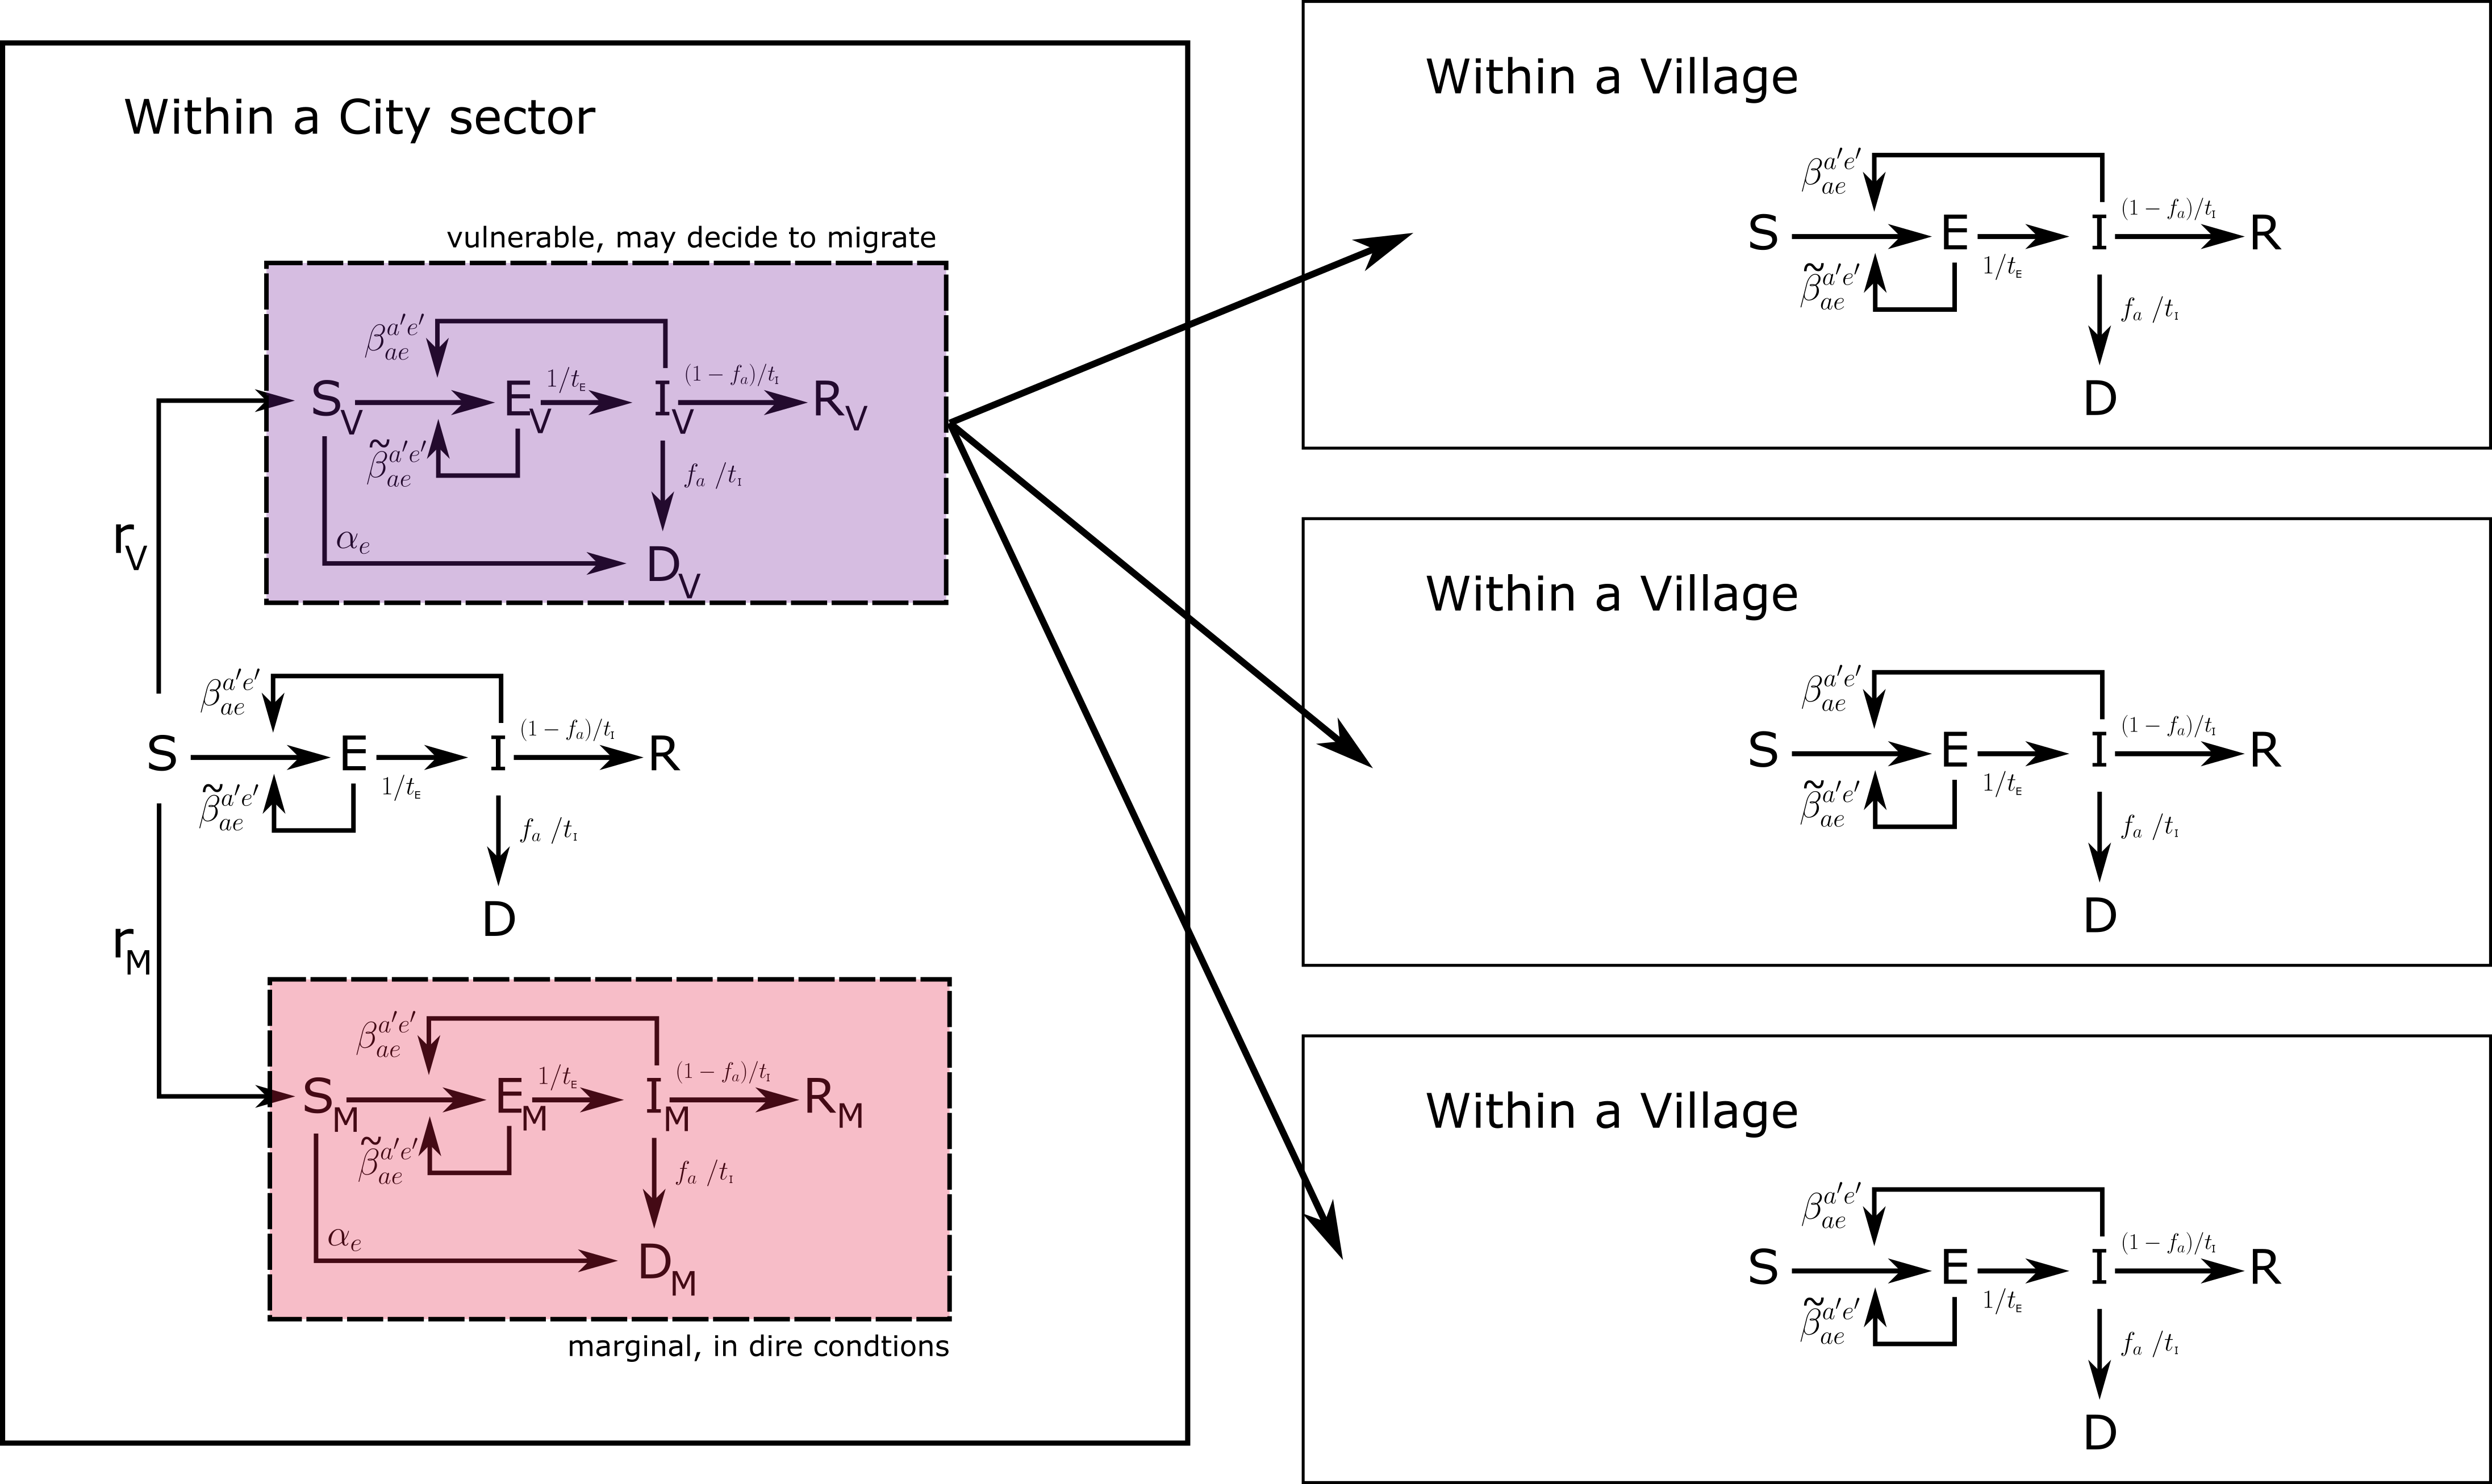
\includegraphics[width=\textwidth]{scheme2-network}
\end{figure}


and the corresponding equations within each module are

\begin{eqnarray}
\dbdt S_{ae} &=& - S_{ae}(t) \sum_{a',e'} \bigg( \beta^{ae}_{a'e'}(t) \frac{I_{a'e'}(t)}{N_{a'e'}(t)} + \tilde{\beta}^{ae}_{a'e'}(t) \frac{E_{a'e'}(t)}{N_{a'e'}(t)} \bigg) + \mathcal{M}^{S}_{ae}(t)\\
\dbdt E_{ae} &=& S_{ae}(t) \sum_{a',e'} \bigg( \beta^{ae}_{a'e'}(t) \frac{I_{a'e'}(t)}{N_{a'e'}} + \tilde{\beta}^{ae}_{a'e'}(t) \frac{E_{a'e'}(t)}{N_{a'e'}} \bigg) - E_{ae}(t)/t_E + \mathcal{M}^{E}_{ae}(t)\\
\dbdt I_{ae} &=& E_{ae}(t)/t_E - I_{ae}(t)/t_I + \mathcal{M}^{I}_{ae}(t)\\     
\dbdt R_{ae} &=& (1- f_{a}) I_{ae}(t)/t_I  + \mathcal{M}^{R}_{ae}(t)\\
\dbdt D_{ae} &=& f_{a} I_{ae}(t)/t_I + \alpha_e S_{ae}(t)
\end{eqnarray}
and the intermodule transitions are absorbed in to $\mathcal{M}$. 

Notice that the parameters are dependent on age (a) and economic (e) category too.

\begin{table}[H]
	\centering
	\begin{tabular}{l r} % c l}
		\toprule
		\textbf{Parameter} & \textbf{Symbol} \\ % & \textbf{Value} & \textbf{Units} \\
		\midrule
		interactions rate between $S_{ae}$ and $E_{a'e'}$ & $\beta^{ae}_{a'e'}$ \\ 
		interactions rate between $S_{ae}$ and $I_{a'e'}$ & $\tilde{\beta}^{ae}_{a'e'}$ \\ 
		rate of deaths due to economic reasons (depends on economic category)  & $\alpha_e$ \\
		time spent in E (latency period) & $t_E$ \\ 
		time spent in I (infectious period) & $t_I$ \\
		proportion for which the disease is fatal (depends on age category) & $f_a$ \\
		transitions between modules & $\mathcal{M}$ \\
		\bottomrule
	\end{tabular}
	\caption{Parameters in our model}
	\label{table:our_model_parameters}
\end{table}
The epidemiological parameters, $f_a, t_E, t_I$ have been taken from \cite{NeherFeb2020}. The rate of infection and economic death rate had to be deciphered from social contact maps \cite{Keisha2017} and reports of poverty-related deaths in India.
The social contact map of India presented by Keisha et al is for 16 age categories and is described by a 16x16 matrix. For, our purposes, this had to be convolved with the age distribution of India to obtain a 3x3 matrix, $ C_{a'}^a$. Economic categories were not considered in the study. We therefore defined $\beta$ in the following manner:
\begin{enumerate}
	\item within an economic group, i.e. $e' = e$, social contact map is as given in the study by Keisha et al, $\beta^{ae}_{a'e} = \lambda C_{a'}^a$. $\lambda$ stands for the probability of infection on contact.
	\item rich-poor interactions are limited to the young, $\beta^{a,2}_{a',2} = 0.5 \lambda C_{a'}^a$
	\item in all other cases, the degree of contact is zero.
\end{enumerate}

With the above layout in place, we perform a few quick checks on the parameters. 
\begin{figure}[H]
	\centering
	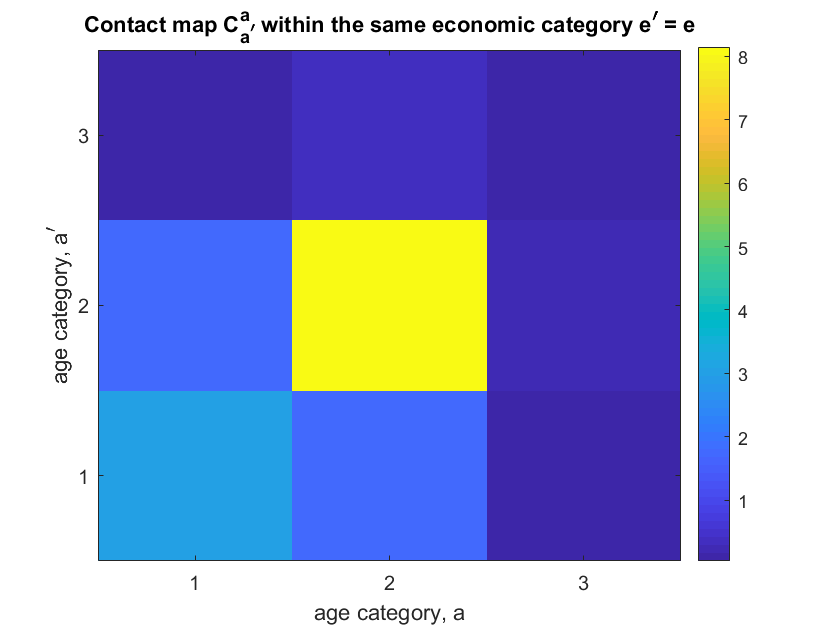
\includegraphics[width=0.6\textwidth]{ContactMap}
\end{figure}

In principle the number of S-E contacts would be much larger than S-I contacts and therefore we will take $\tilde{\beta} = \gamma \beta$, where $0 \leq \gamma \leq 1$. Mitigation strategies bring down the amount of interactions, i.e. $\beta \to \beta \zeta$, where $0 \leq \zeta \leq 1$. According to some reports, India has 2.5 million poverty-related deaths in a year \cite{}. This means that without mitigation strategies in place, \[ \sum_{e=1}^{2} \alpha_e^o \sim \frac{2.5 \times 10^6}{365} \text{per day}, \quad \alpha_3 = 0 \:\: \text{i.e. rich are not affected} \] However, mitigation strategies like lock-down are going to increase this rate as more poor people are likely to fall off the grid without being able to commute to work daily. For the time being, we factor this in as, \[ \alpha_e = \frac{\alpha^o_e}{\zeta^n} \] where $\alpha_e^o = 2.2 \times 10^{-3}$ per day.
A more sophisticated model is to be discussed.

With the above layout in place, we perform a few quick checks on the parameters. 
\begin{figure}[H]
	\centering
	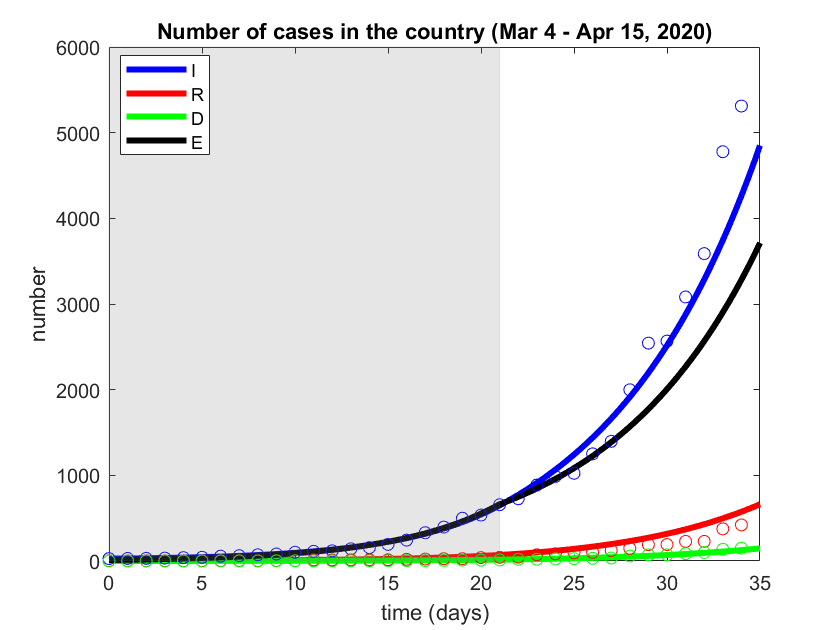
\includegraphics[width=0.7\textwidth]{model_data_comparison}
	\caption{A comparison of simulations to the real data obtained from JHU CSSE \cite{JHUdata}. Initial number of infectious (I) cases were 28 on Mar 4, 2020 and we assumed that the number of exposed (E) people were 12 (about 0.4 times the number of infectious cases). We also assumed that all the inital cases belonged to the young , rich category. Lock-down is implemented on Mar 25, 2020. Parameters used for simulation (NOT best fit): $t_E = 5$, $t_I = 42$, $ f_a = [0.0910, 0.1867, 0.6194] $, $\lambda = 0.019$, $\gamma = 0$, $\zeta = 0.85$.  }
\end{figure}

\pagebreak
\subsection{Case: absence of economic module in the model, $\alpha_e = 0$}

\begin{figure}[H]
	\centering
	\begin{subfigure}[b]{0.5\textwidth}
		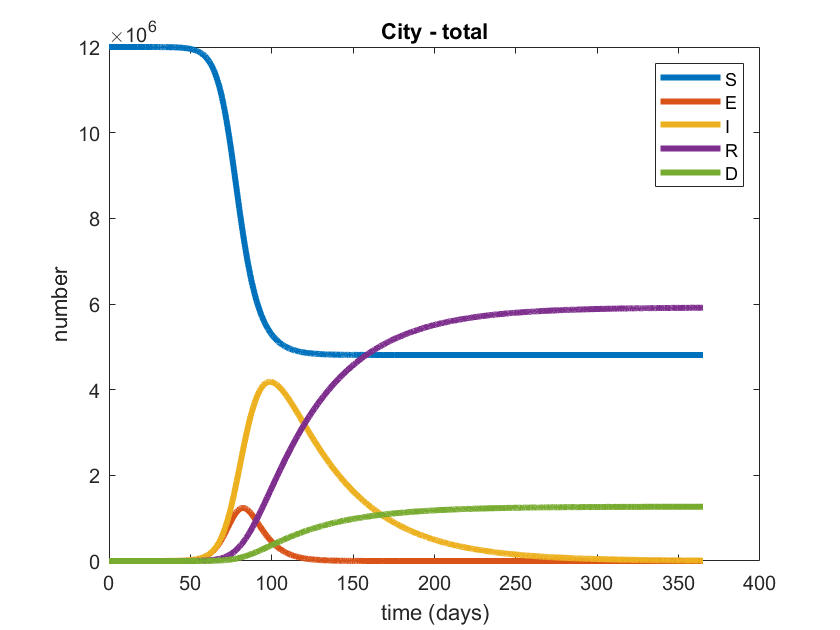
\includegraphics[width=\textwidth]{no-economic-effect/no-mitigation/City-total}
	\end{subfigure}%
	\begin{subfigure}[b]{0.5\textwidth}
		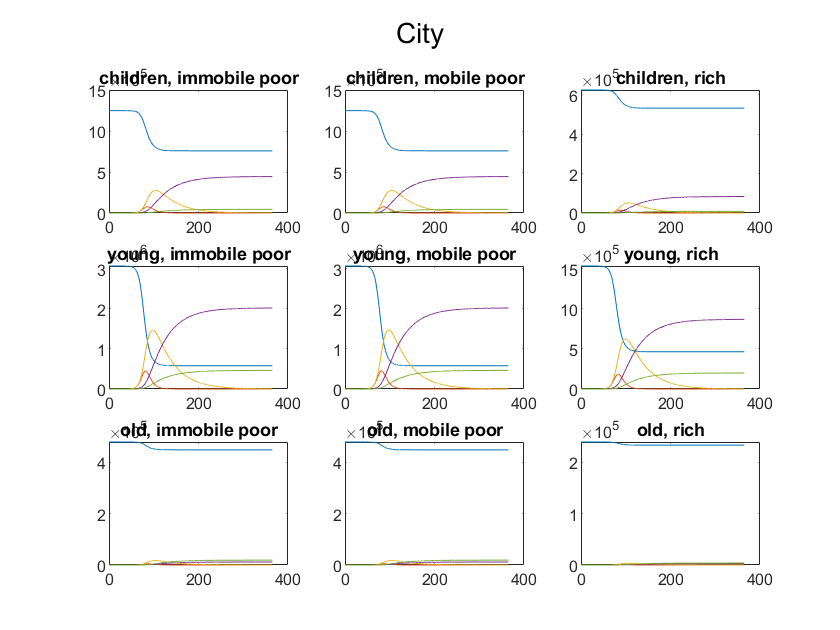
\includegraphics[width=\textwidth]{no-economic-effect/no-mitigation/City-all-cat}
	\end{subfigure}

	\begin{subfigure}[b]{0.5\textwidth}
		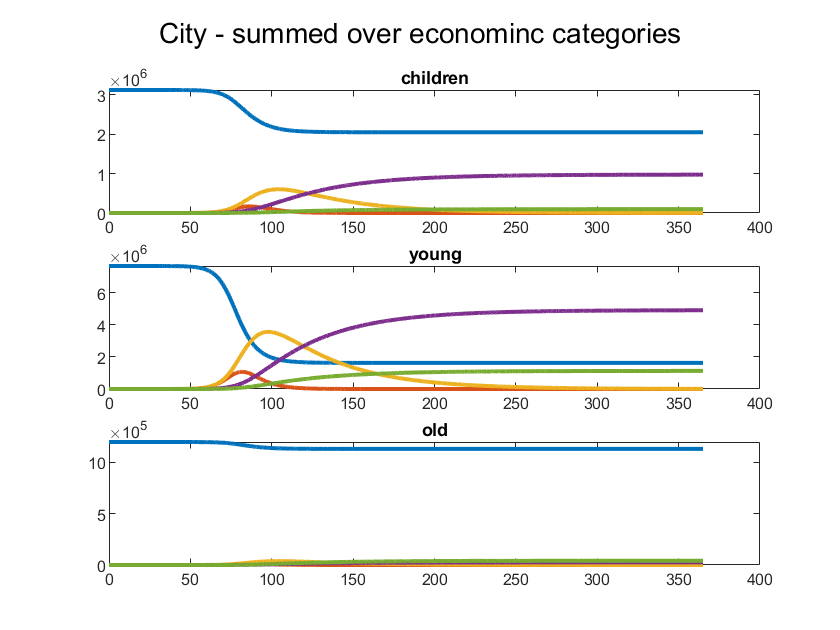
\includegraphics[width=\textwidth]{no-economic-effect/no-mitigation/City-age-cat}
	\end{subfigure}%
	\begin{subfigure}[b]{0.5\textwidth}
		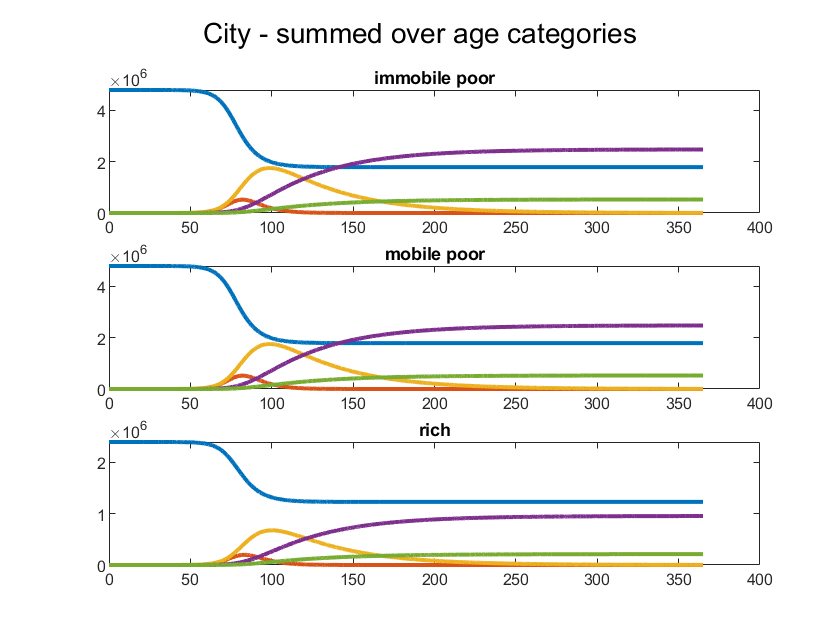
\includegraphics[width=\textwidth]{no-economic-effect/no-mitigation/City-eco-cat}
	\end{subfigure}

	\caption{Without mitigation strategies, i.e. $\zeta = 1$ throughout. For full-size images here: \url{here}.}
\end{figure}

\begin{figure}[H]
	\centering
	\begin{subfigure}[b]{0.5\textwidth}
		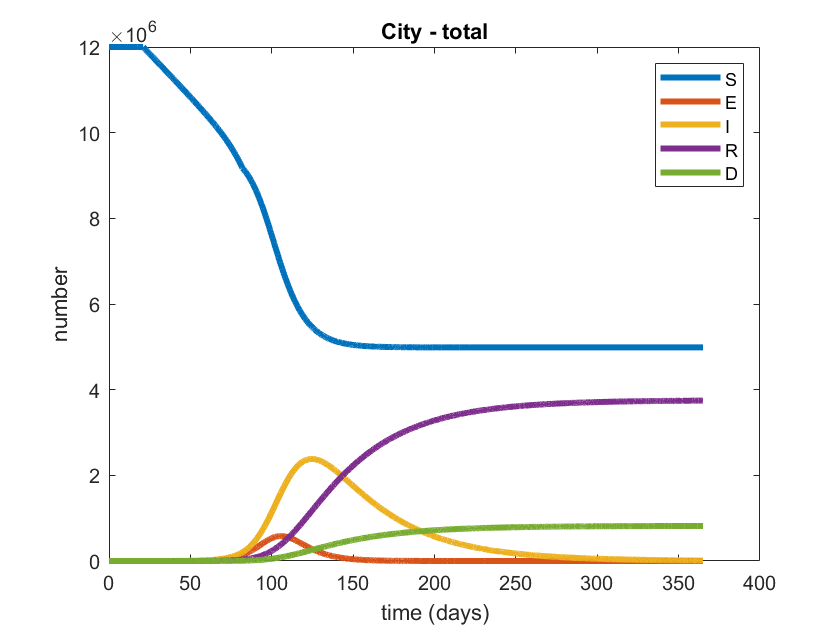
\includegraphics[width=\textwidth]{no-economic-effect/weak-mitigation/City-total}
	\end{subfigure}%
	\begin{subfigure}[b]{0.5\textwidth}
		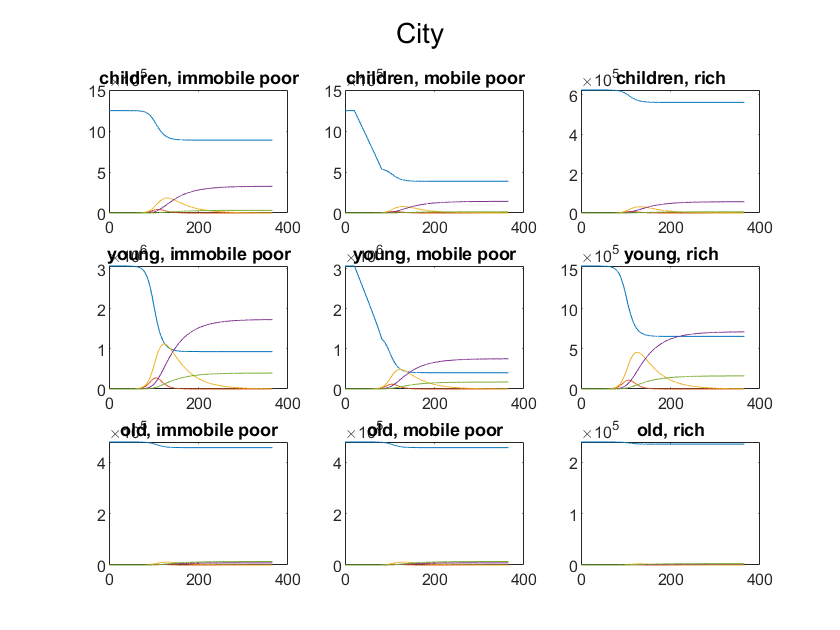
\includegraphics[width=\textwidth]{no-economic-effect/weak-mitigation/City-all-cat}
	\end{subfigure}
	
	\begin{subfigure}[b]{0.5\textwidth}
		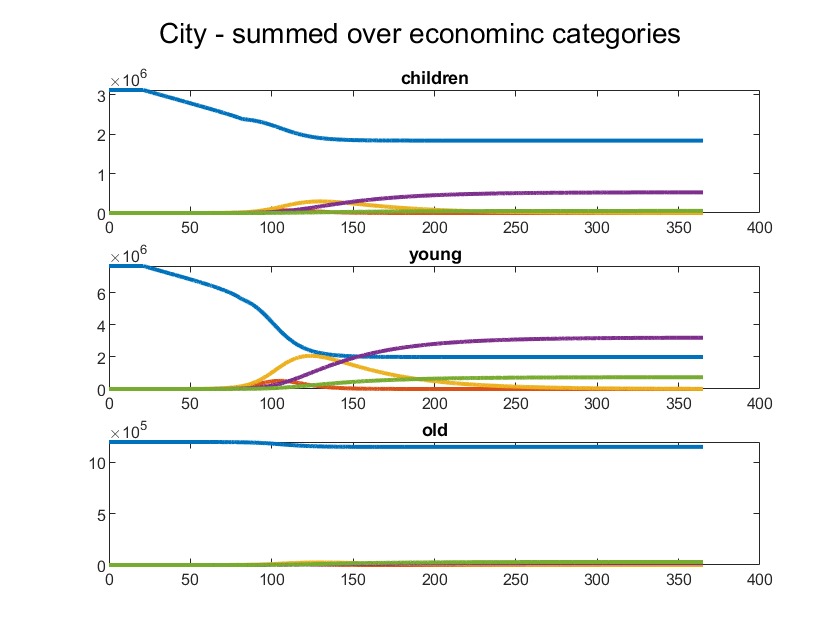
\includegraphics[width=\textwidth]{no-economic-effect/weak-mitigation/City-age-cat}
	\end{subfigure}%
	\begin{subfigure}[b]{0.5\textwidth}
		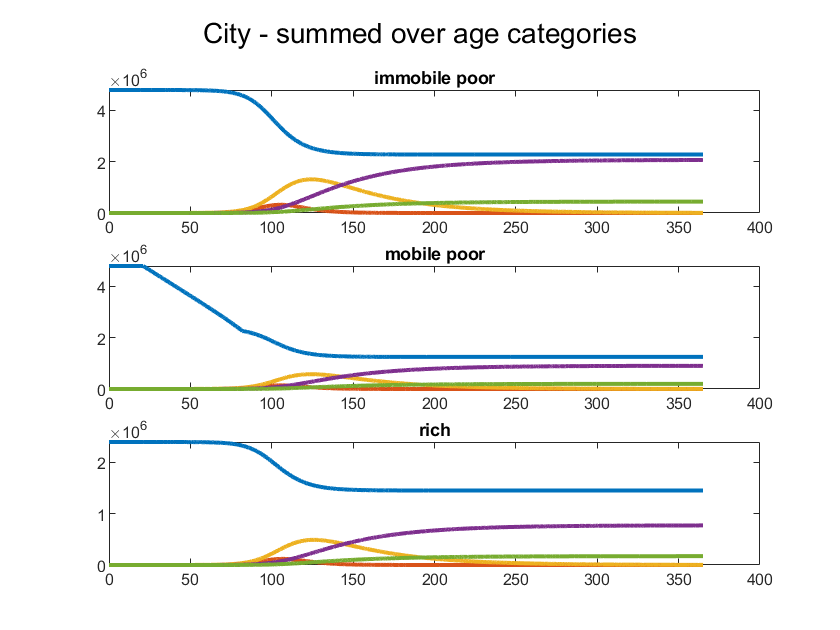
\includegraphics[width=\textwidth]{no-economic-effect/weak-mitigation/City-eco-cat}
	\end{subfigure}

	\begin{subfigure}[b]{0.5\textwidth}
		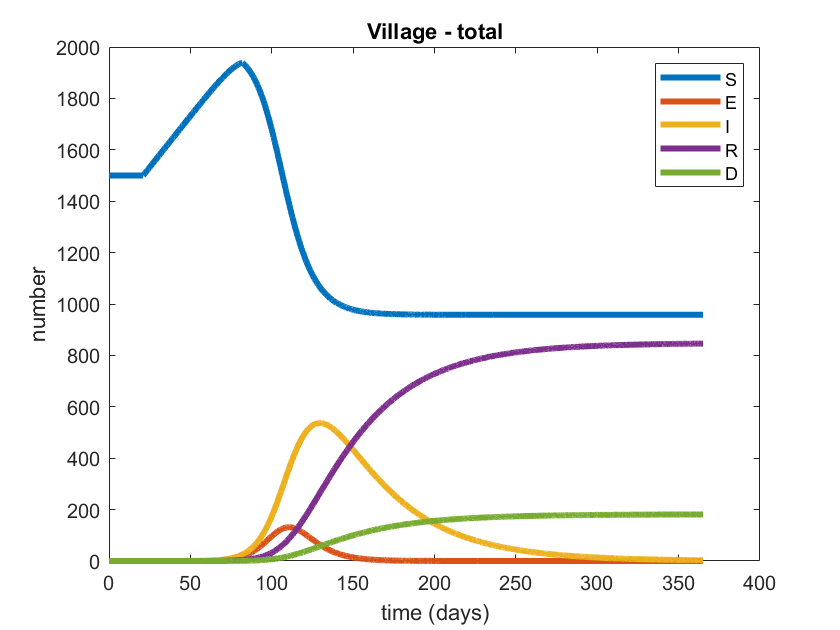
\includegraphics[width=\textwidth]{no-economic-effect/weak-mitigation/Village-total}
	\end{subfigure}%
	\begin{subfigure}[b]{0.5\textwidth}
		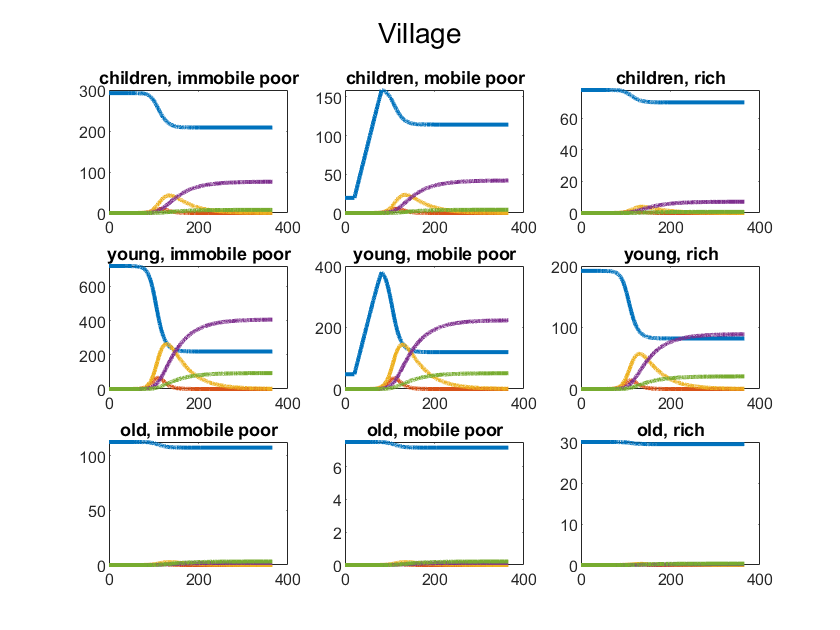
\includegraphics[width=\textwidth]{no-economic-effect/weak-mitigation/Village-all-cat}
	\end{subfigure}
	
	\begin{subfigure}[b]{0.5\textwidth}
		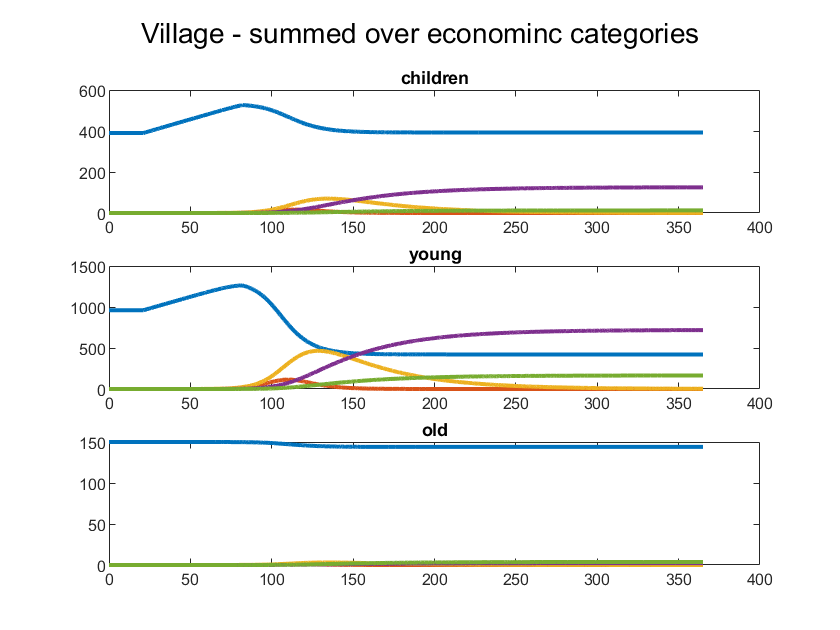
\includegraphics[width=\textwidth]{no-economic-effect/weak-mitigation/Village-age-cat}
	\end{subfigure}%
	\begin{subfigure}[b]{0.5\textwidth}
		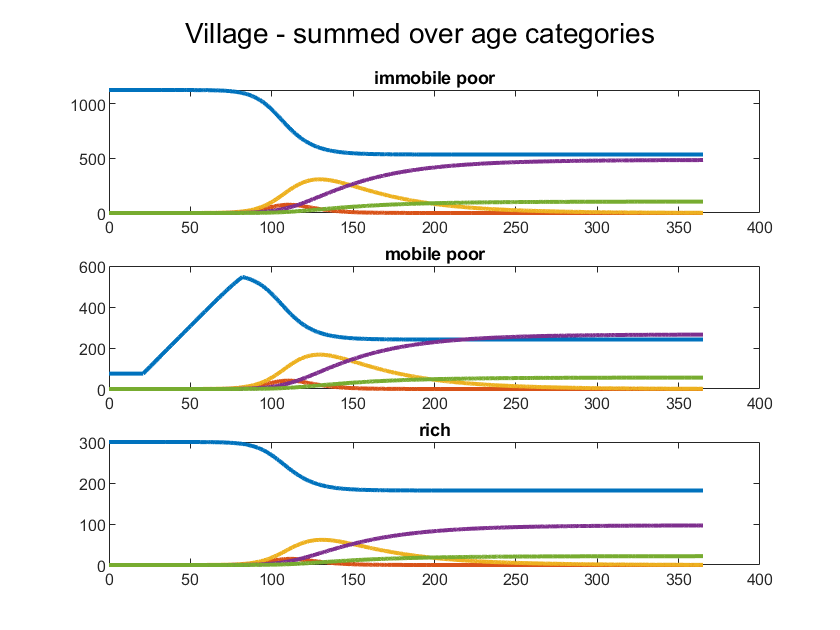
\includegraphics[width=\textwidth]{no-economic-effect/weak-mitigation/Village-eco-cat}
	\end{subfigure}
	
	\caption{With mitigation strategy implemented 21 days after $t = 0$, i.e. $\zeta = 1$ for $t \leq 21$, and $ \zeta = 0.85$ for $t > 21$. For full-size images here: \url{here}.}
\end{figure}


\begin{figure}[H]
	\centering
	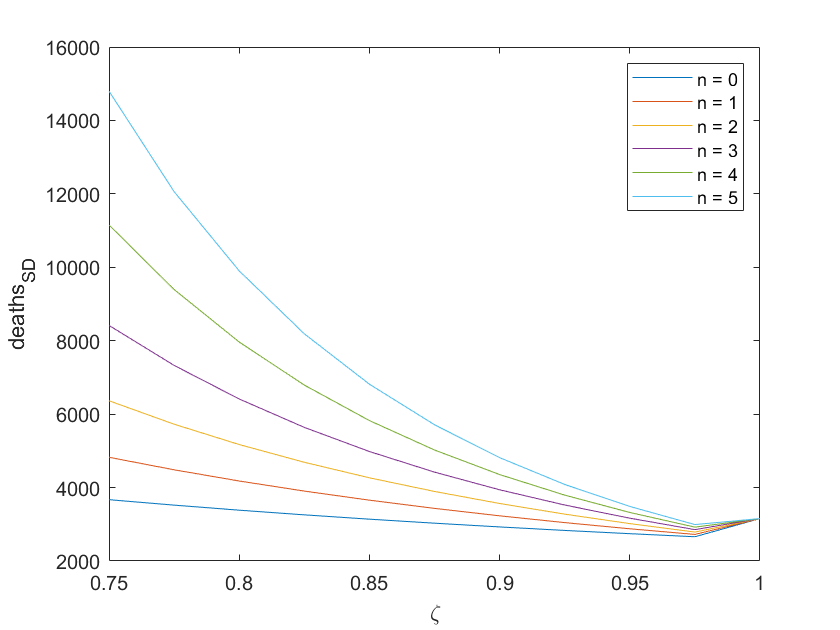
\includegraphics[width=\textwidth]{/economic-model1/deaths_SD}
\end{figure}


\begin{figure}[H]
	\centering
	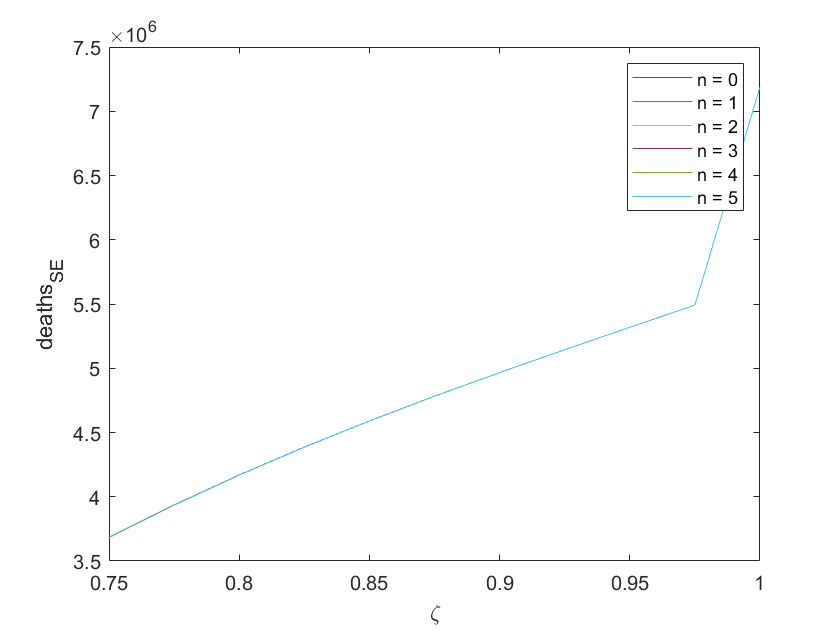
\includegraphics[width=\textwidth]{/economic-model1/deaths_ID}
\end{figure}


\begin{figure}[H]
	\centering
	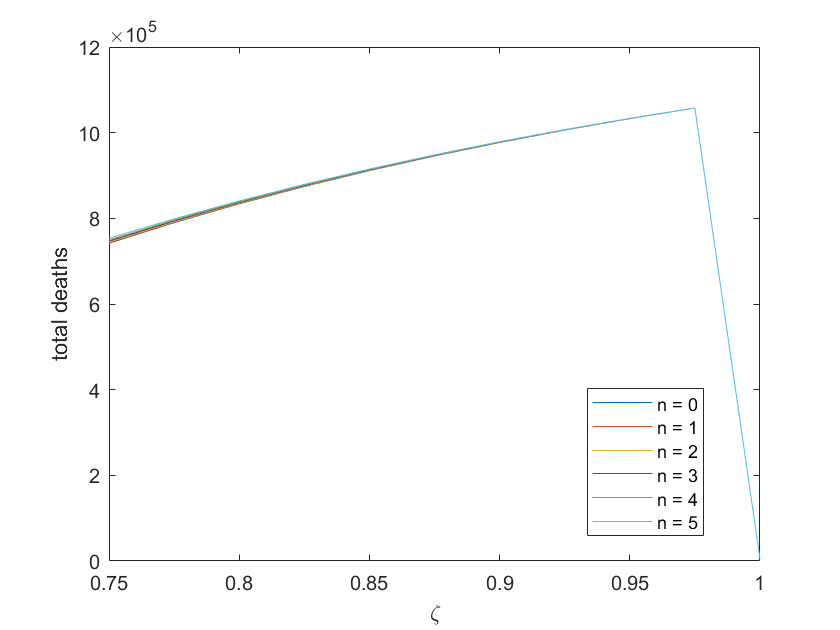
\includegraphics[width=\textwidth]{/economic-model1/total_deaths}
\end{figure}

\pagebreak
Things to-do:

\begin{enumerate}
	\item \textcolor{red}{parameters and their toggles}
	
	\item \textcolor{red}{the economic module is fairly simple and the model is giving obvious results. Discuss with Amit.}
	
	\item \textcolor{red}{differences in the public health infrastructure: $f_a$ different in villages and city? or infections in villages cause migration back to city. }
	
	\item \textcolor{red}{having a social net might ensure $\alpha_e$ does not ramp up due to mitigation and migration also does not play a strong role in that case}
	
\end{enumerate}



\subsection{Take home messages - summarize results}

\begin{thebibliography}{10} 
	
	\bibitem{NeherFeb2020} \url{https://neherlab.org/covid19/about}

	\bibitem{Keisha2017} Prem, Kiesha, Alex R. Cook, and Mark Jit. "Projecting social contact matrices in 152 countries using contact surveys and demographic data." PLoS computational biology 13.9 (2017): e1005697.
	
	\bibitem{JHUdata} \url{https://github.com/CSSEGISandData/COVID-19}
	
\end{thebibliography}








\end{document}          